\documentclass[a4paper,12pt]{article} 

%%% Работа с русским языком
\usepackage{cmap}                           % поиск в PDF
\usepackage{mathtext} 			 	       % русские буквы в формулах
\usepackage[T2A]{fontenc}               % кодировка
\usepackage[utf8]{inputenc}              % кодировка исходного текста
\usepackage[english,russian]{babel}  % локализация и переносы
\usepackage[left=2cm,right=2cm,
    top=2cm,bottom=3cm,bindingoffset=0cm]{geometry}
\usepackage{wrapfig}
\usepackage{gensymb}
\usepackage{textcomp}
\usepackage{multirow}
\usepackage{amsmath,amsfonts,amssymb,amsthm,mathtools} % AMS
\usepackage{euscript}	 % Шрифт Евклид
\usepackage{mathrsfs} % Красивый матшрифт
\usepackage{graphicx}%Вставка картинок правильная
\usepackage{float}%"Плавающие" картинки
\usepackage{wrapfig}%Обтекание фигур (таблиц, картинок и прочего)
\title{Лабораторная работа 3.2.8

Релаксационные колебания}
\author{Кагарманов Радмир Б01-106}
\date{20 декабря 2022 г.}

\begin{document}
\maketitle
\thispagestyle{empty}
\newpage
\setcounter{page}{1}

\paragraph{Цель работы:} изучение вольт-амперной характеристики нормального тлеющего разряда; исследование релаксационных колебаний генератора на стабилитроне.

\paragraph{В работе используется:} стабилитрон СГ-2 (газонаполненный диод) на монтажной плате, магазин ёмкостей, магазин сопротивлений, источник питания, амперметр, вольтметр, осциллограф.

\paragraph{Описание\\}
В работе исследуются релаксационные колебания, возбуждаемые в электрическом контуре, состоящем из $C$, резистора $R$ и газоразрядного диода с $S$-образной вольт-амперной характеристикой. Релаксационные колебания в этом случае являются совокупностью двух апериодических процессов - зарядки конденсатора и его разрядки. В нашей установке роль <<ключа>>, обеспечивающего попеременную зарядку и разрядку конденсатора, играет газоразрядный диод. Зависимость тока от напряжения на газоразрядной лампе $I_{S}(V)$ не подчиняется закону Ома. Ток в лампе возникает только в том случае, если разность потенциалов на её электродах достигает напряжения зажигания $V_1$. При этом скачком устанавливается конечная сила тока $I_1$ - в лампе возникает нормальный текущий разряд. при дальнейшем незначительном увеличении напряжения $V$ сила тока заметно возрастает по закону, близкому к линейному.\par 
Если начать уменьшать напряжение на горящей лампе, то при напряжении, равном $V_1$, лампа ещё не гаснет, и сила тока продолжает уменьшаться. Лампа перестаёт пропускать ток лишь при напряжении гашения $V_2$, которое обычно существенно меньше $V_1$. Сила тока при этом скачком падает от значения $I_2$, меньшего $I_1$, до нуля. \par
Схема экспериментального стенда для изучения релаксационных колебаний представлена на рис. 1. 

\begin{figure}[!h]
\centering
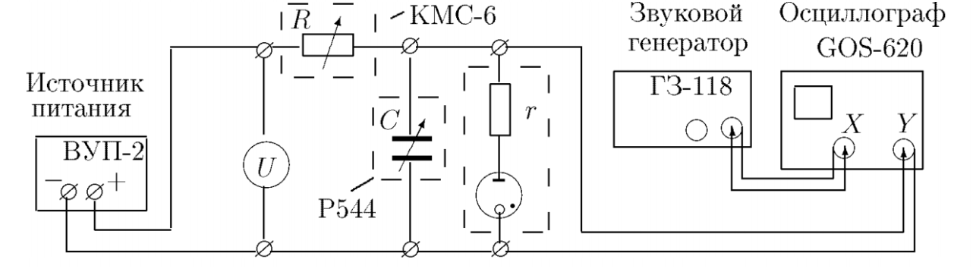
\includegraphics[width=0.9\linewidth]{установка.png}
\caption{Экспериментальная установка}
\label{fig:mpr}
\end{figure}

На рис. 2 представлены релаксационные колебания.
\begin{figure}[!h]
\centering
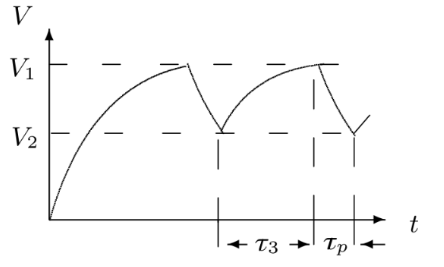
\includegraphics[width=0.6\linewidth]{Релаксационные.png}
\caption{Релаксационные колебания}
\label{fig:mpr}
\end{figure}
Они будут проходить с амлитудой $V_1 - V_2$. Полное время периода колебаний $T$ состоит из суммы времени зарядки и времени разрядки Во время зарядки конденсатора лампа не горит($I(V)=0$), и уравнение для напряжения $V(t)$ принимает вид
\begin{equation}
    RC\frac{dV}{dt}=U-V.
\end{equation}
Будем отсчитывать время с момента гашения лампы. Решив уравнение (1), найдём:
\begin{equation}
    V = U - (U-V_2)e^{-t/RC}.
\end{equation}
В момент зажигания $t=\tau_{з}$, $V=V_1$, поэтому
\begin{equation}
    V_1 = U-(U-V_2)e^{-\tau_з /RC}.
\end{equation}
Из уравнений (2) и (3) нетрудно найти период колебаний:
\begin{equation}
    T\approx \tau_з = RCln\frac{U-V2}{U-V1}.
\end{equation}

\paragraph{Обработка результатов}
\subparagraph{1.} Соберём установку, изображённую на рис. 3. Определим напряжения $V_1$ и $V_2$ и построим вольт-амперную характеристику.
\begin{figure}[!h]
\centering
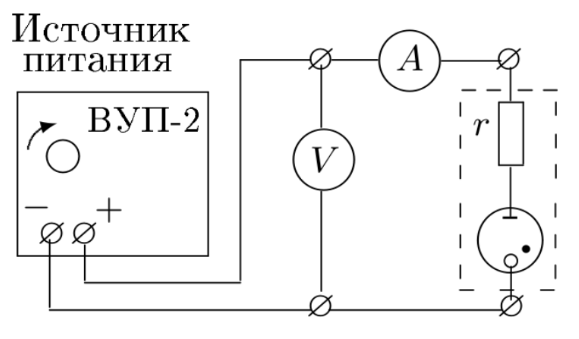
\includegraphics[width=0.6\linewidth]{установка(1).png}
\caption{Экспериментальная установка}
\label{fig:mpr}
\end{figure}

\newpage

\begin{figure}[!h]
\centering
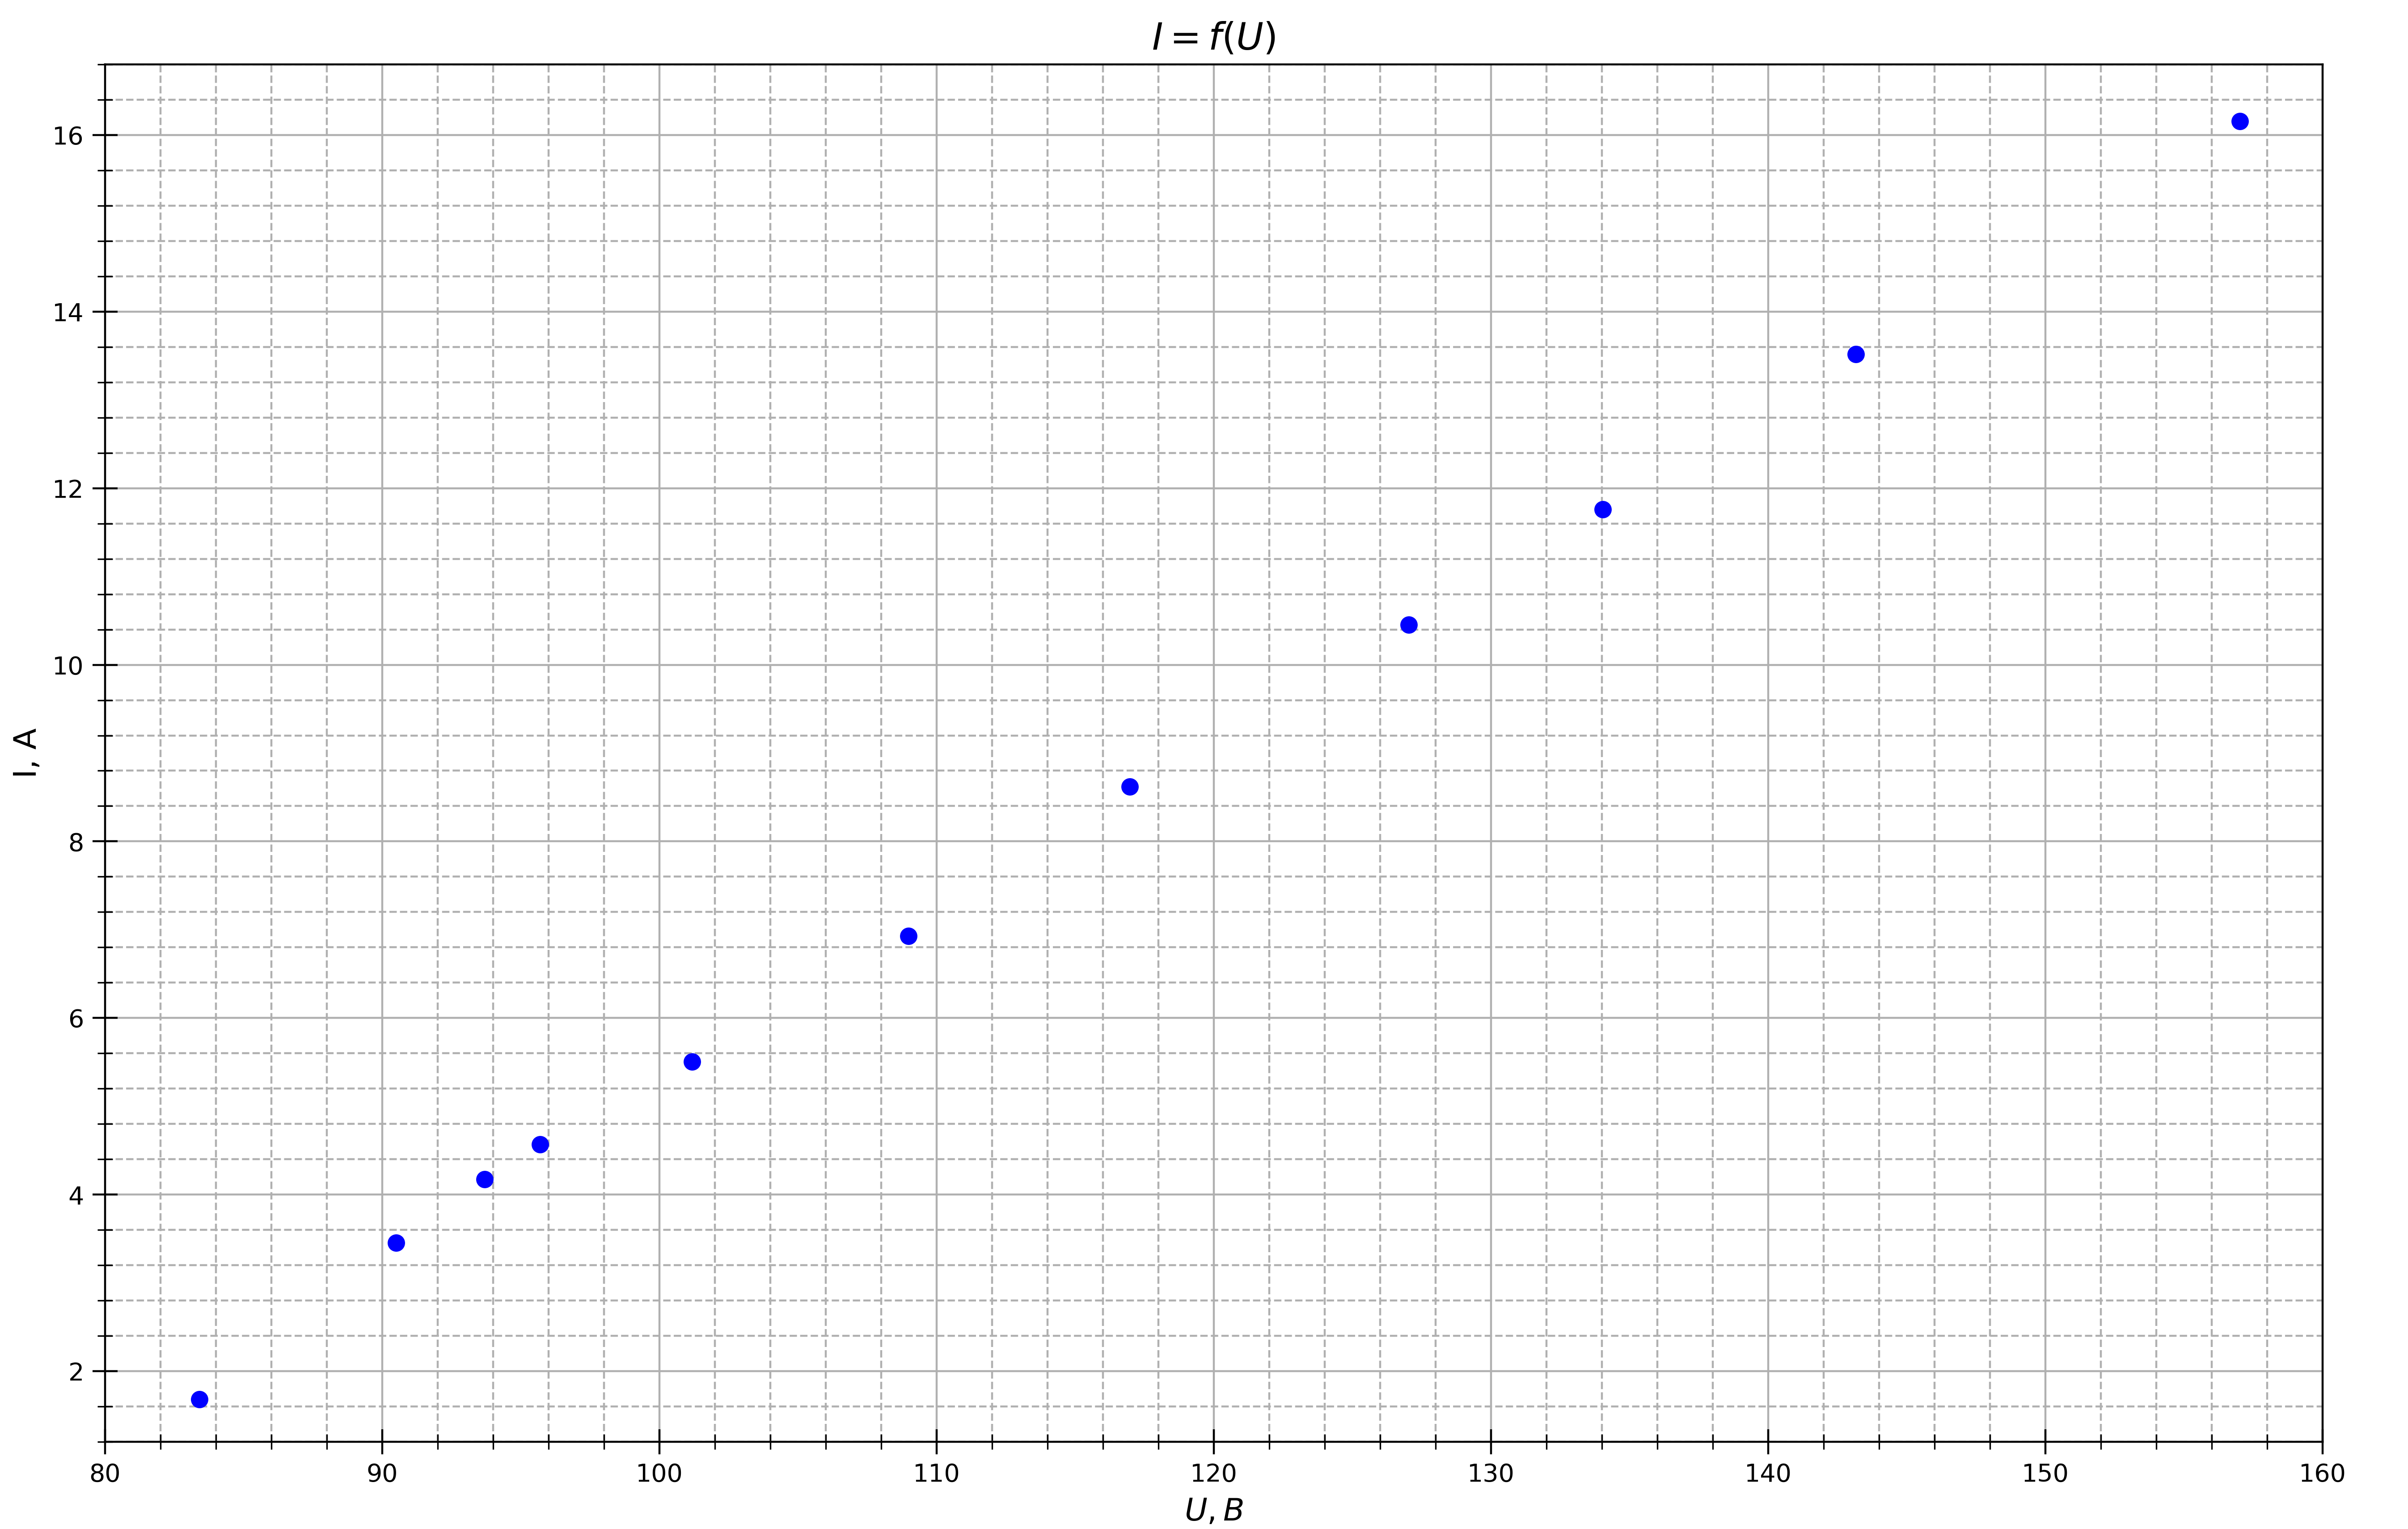
\includegraphics[width=0.6\linewidth]{ВАХ.png}
\caption{Вольт-амперная характеристика}
\label{fig:mpr}
\end{figure}

\begin{center}
    $V_1 = 90,5~В$ и $I_1 = 3,455~А$\\
    $V_2 = 83,4~В$ и $I_2 = 1,680~А$
\end{center}
\subparagraph{2.} Построим графики зависимости периода $T=f(C)$ и $T=f(R)$.
\begin{figure}[!h]
\centering
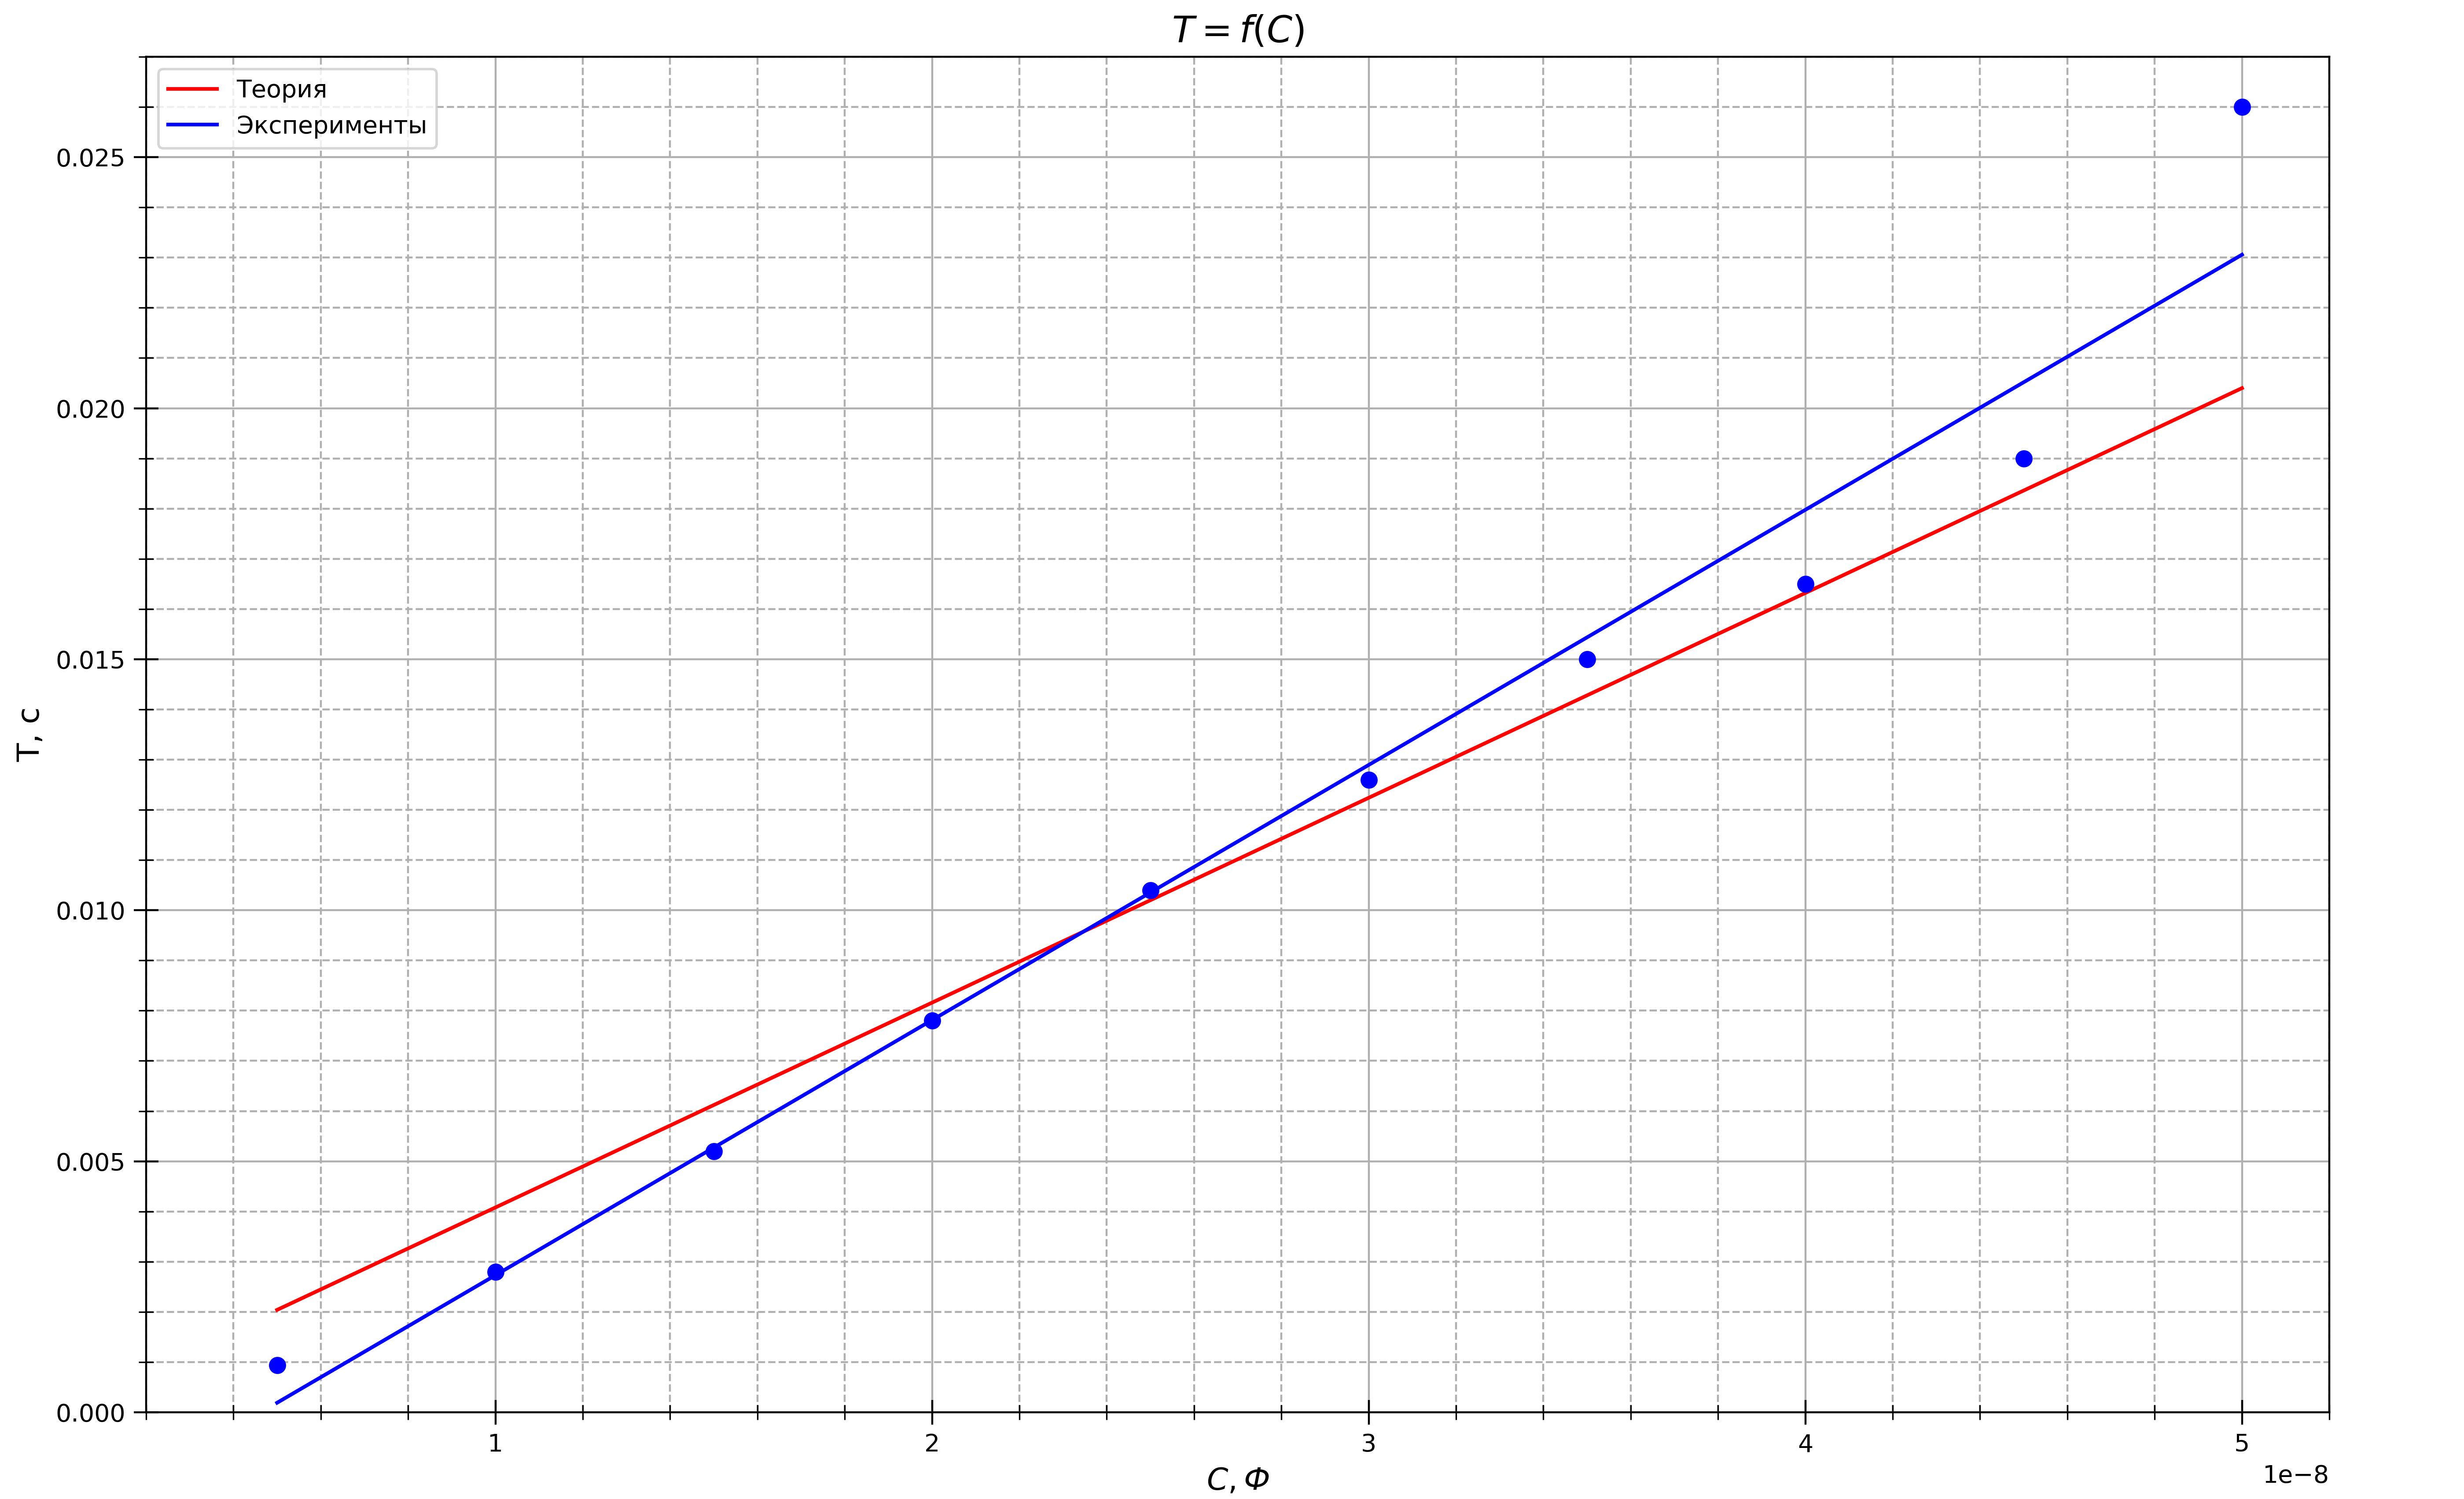
\includegraphics[width=0.7\linewidth]{f(C).png}
\caption{$T=f(C)$}
\label{fig:mpr}
\end{figure}
\newpage
\begin{figure}[!h]
\centering
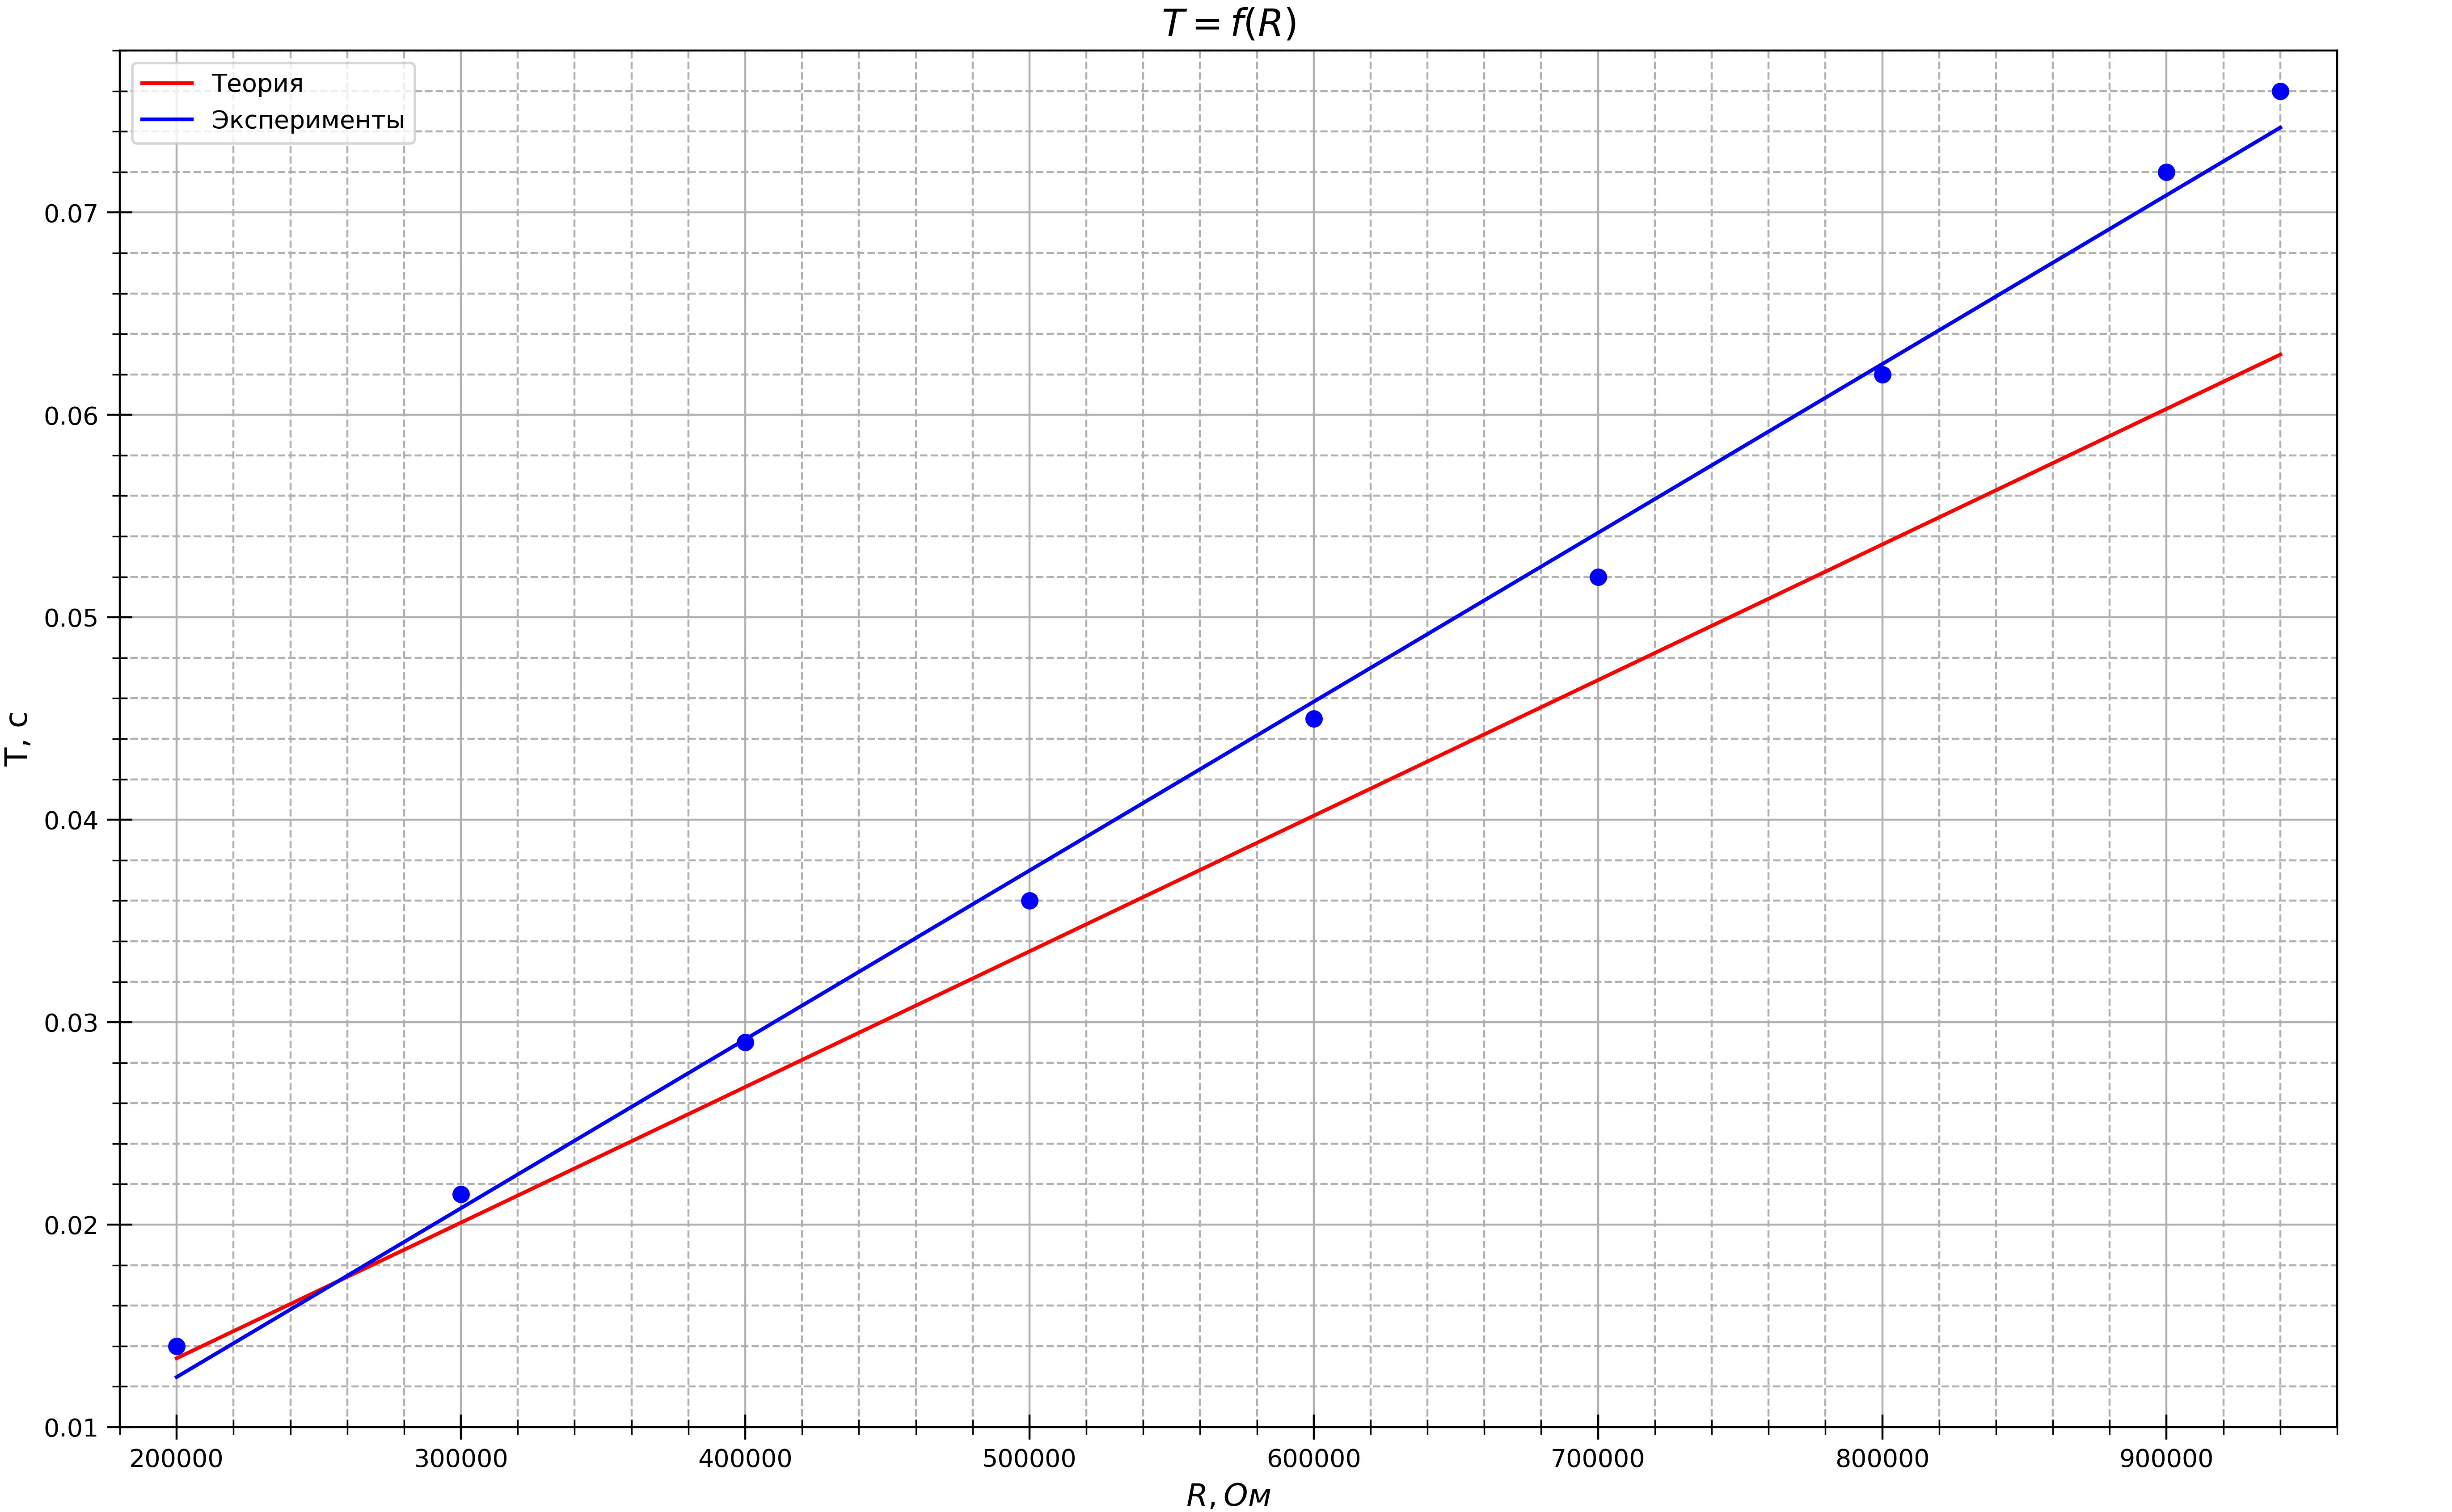
\includegraphics[width=0.7\linewidth]{f(R).png}
\caption{$T=f(R)$}
\label{fig:mpr}
\end{figure}

По графикам видно, что экспериментальные прямые близки к теоретическим.
\paragraph{Вывод:}выполнив данную лабораторную работу, мы изучили вольт-амперную характеристику нормального тлеющего заряда и исследовали релаксационные колебания генератора на стабилитроне. Построили графики зависимости периода $T=f(C)$ и $T=f(R)$, и эксперименты оказались близки к теории.
\end{document}
